
\section{Histogram computation}

\begin{figure}
	\centering
	\subcaptionbox{\emph{boiler}}
	{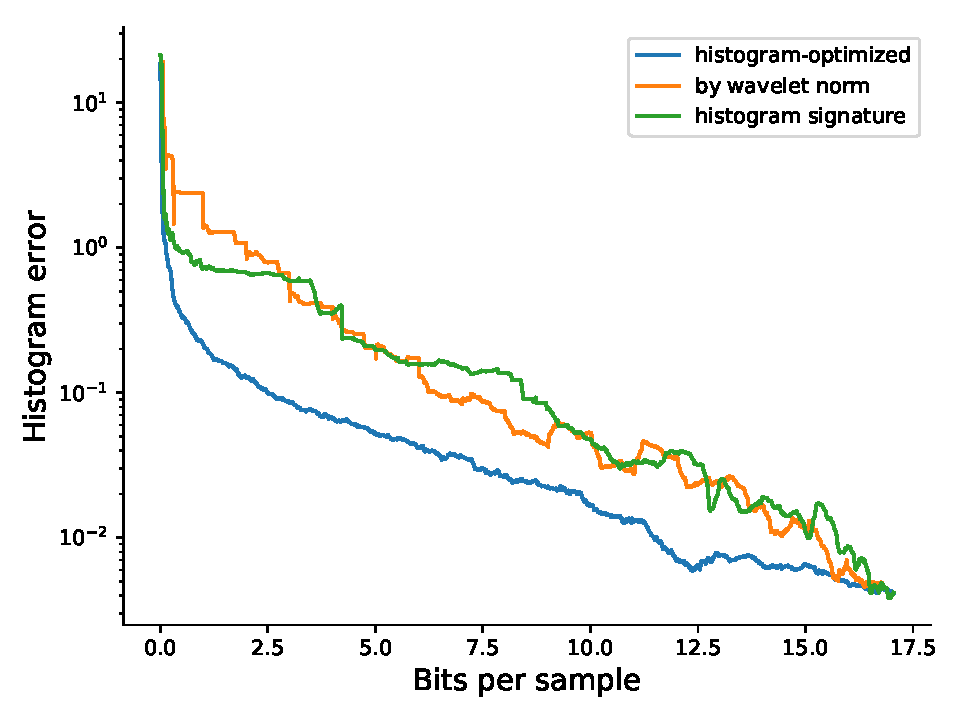
\includegraphics[width=0.48\linewidth]{img/histogram/boiler-histogram.pdf}}
	\subcaptionbox{\emph{boiler, slz}}
	{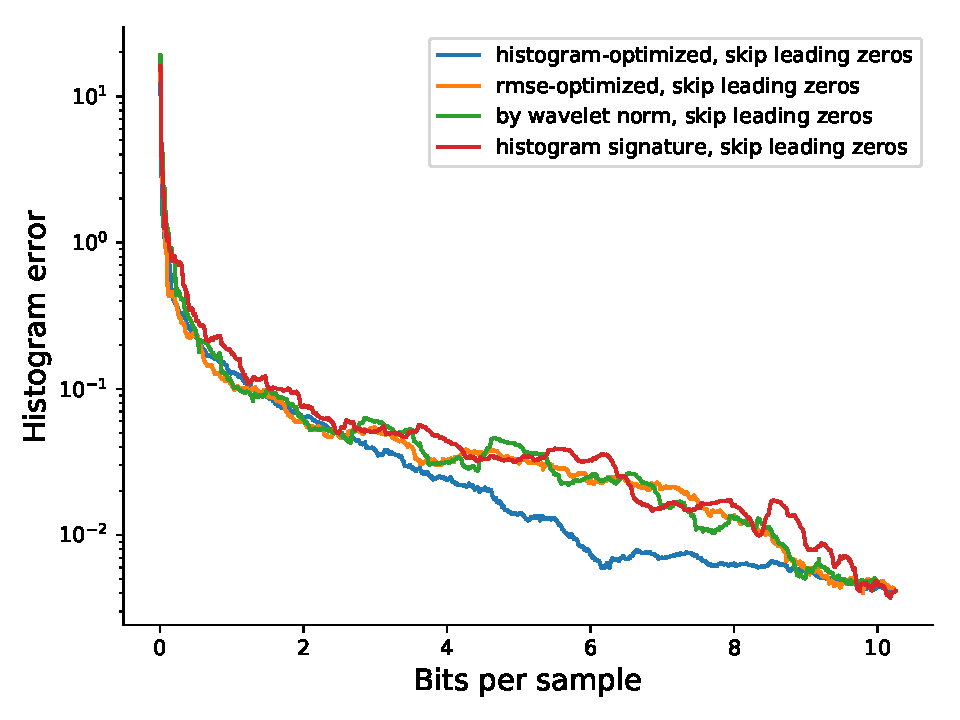
\includegraphics[width=0.48\linewidth]{img/histogram/skip-leading-zeros/boiler-histogram.pdf}}
	\subcaptionbox{\emph{kflame}}
	{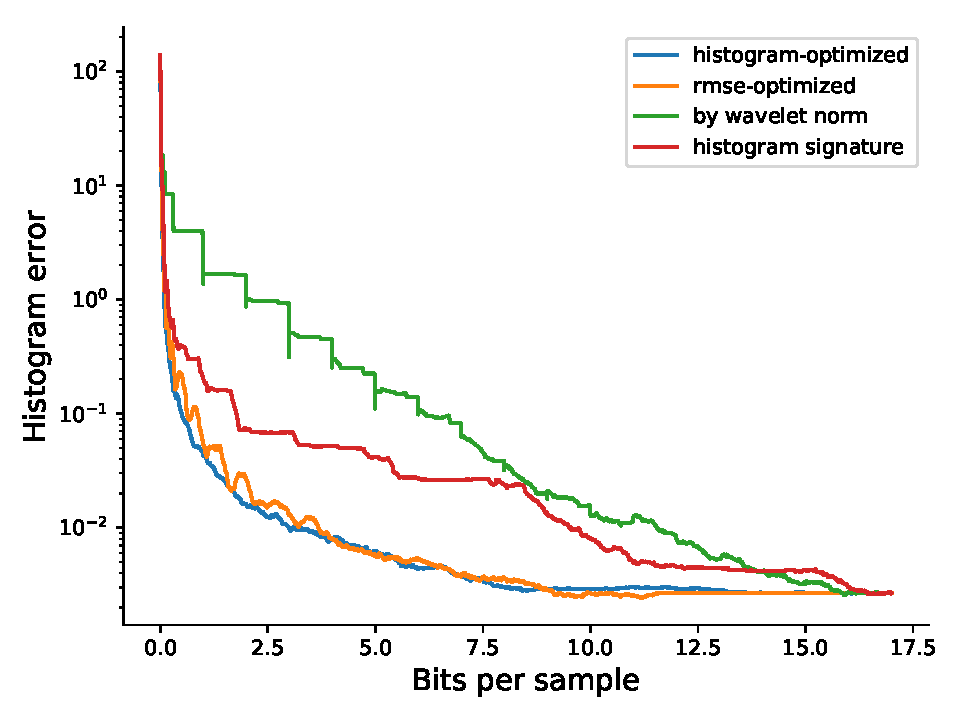
\includegraphics[width=0.48\linewidth]{img/histogram/kflame-histogram.pdf}}
	\subcaptionbox{\emph{kflame, slz}}
	{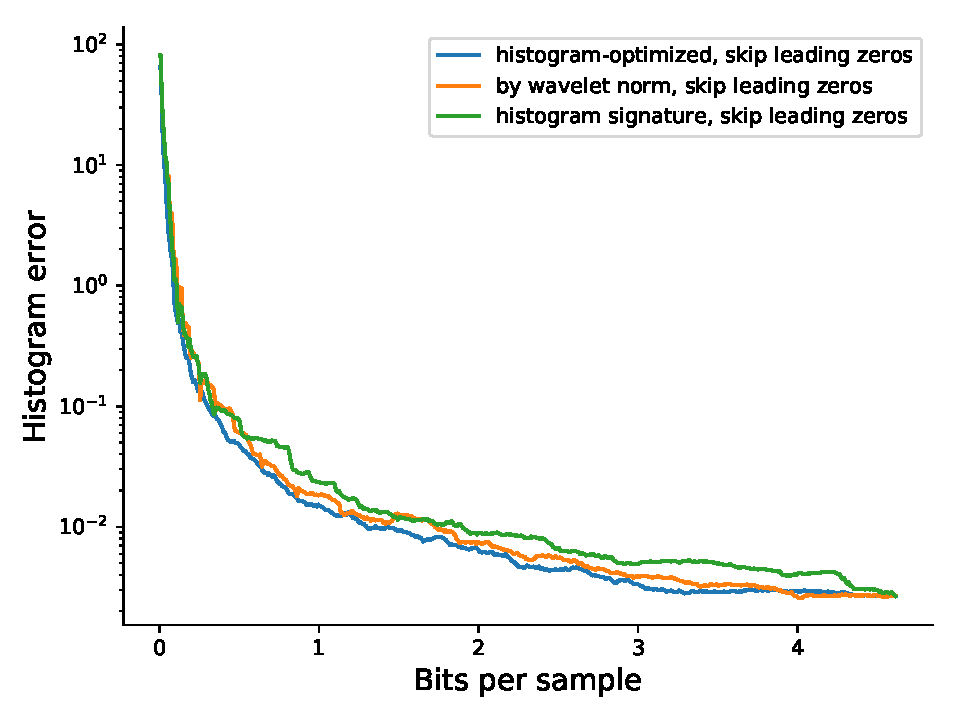
\includegraphics[width=0.48\linewidth]{img/histogram/skip-leading-zeros/kflame-histogram.pdf}}
	\subcaptionbox{\emph{diffusivity}}
	{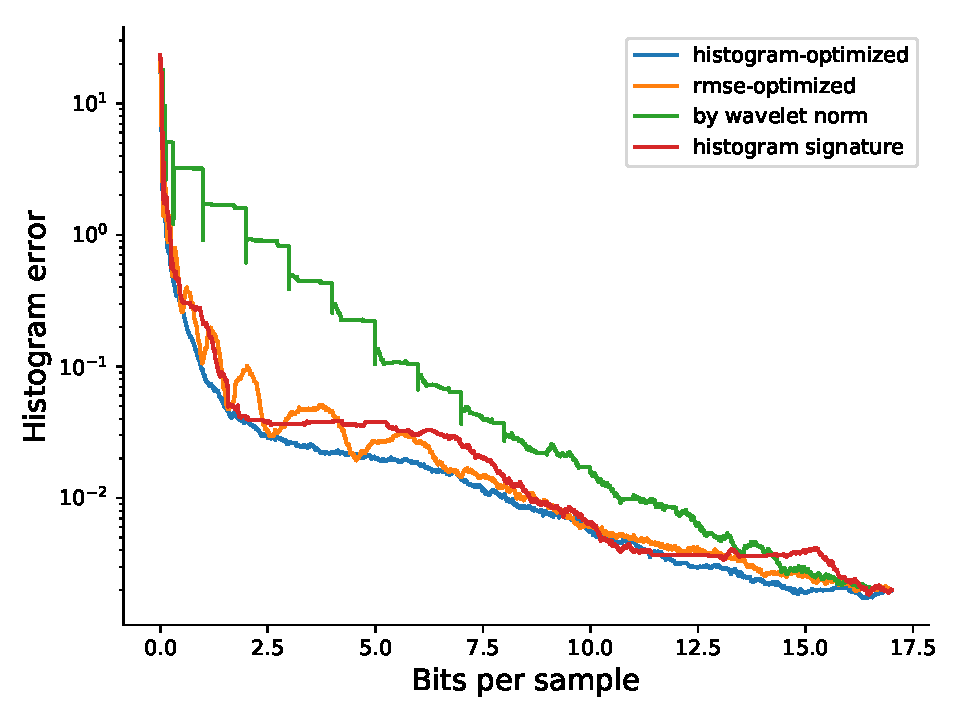
\includegraphics[width=0.48\linewidth]{img/histogram/miranda-diffusivity-histogram.pdf}}
	\subcaptionbox{\emph{diffusivity, slz}}
	{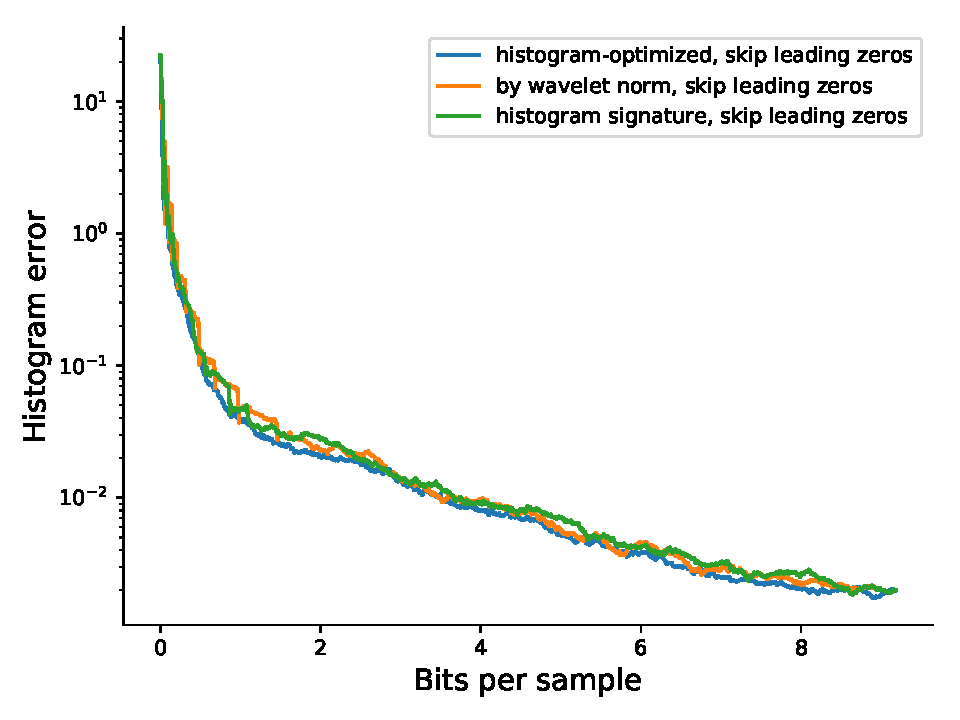
\includegraphics[width=0.48\linewidth]{img/histogram/skip-leading-zeros/miranda-diffusivity-histogram.pdf}}
	\subcaptionbox{\emph{turbulence}}
	{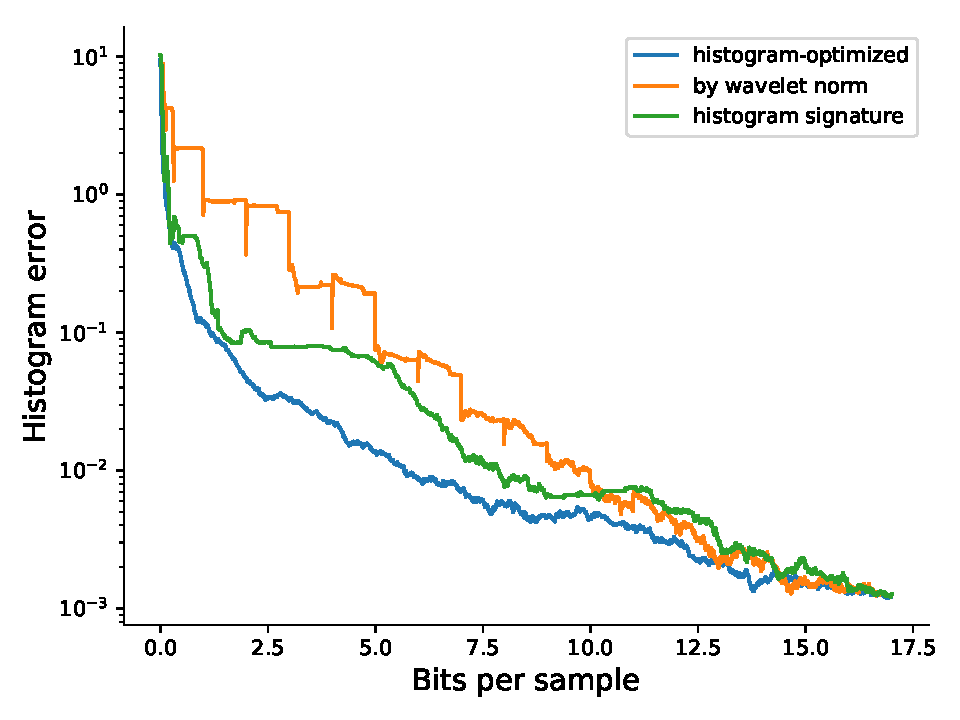
\includegraphics[width=0.48\linewidth]{img/histogram/turbulence-histogram.pdf}}
	\subcaptionbox{\emph{turbulence, slz}}
	{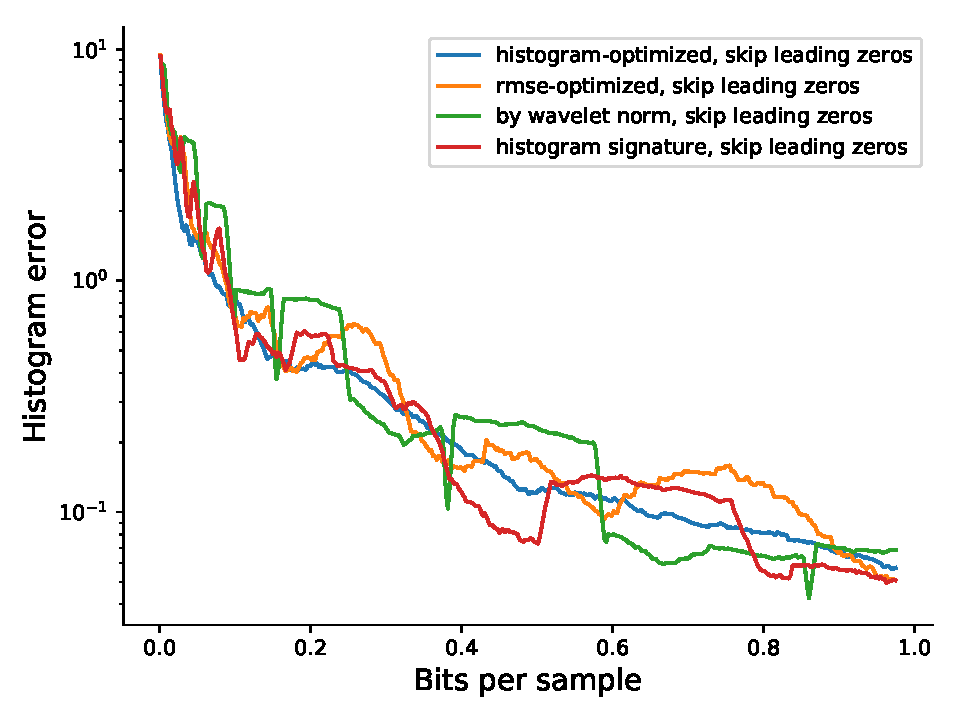
\includegraphics[width=0.48\linewidth]{img/histogram/skip-leading-zeros/turbulence-histogram.pdf}}
	\caption{Histogram comparison.}
	\label{fig:histogram-comparison}
\end{figure}

\begin{figure}
	\centering
	\subcaptionbox{\emph{histogram-optimized}}
	{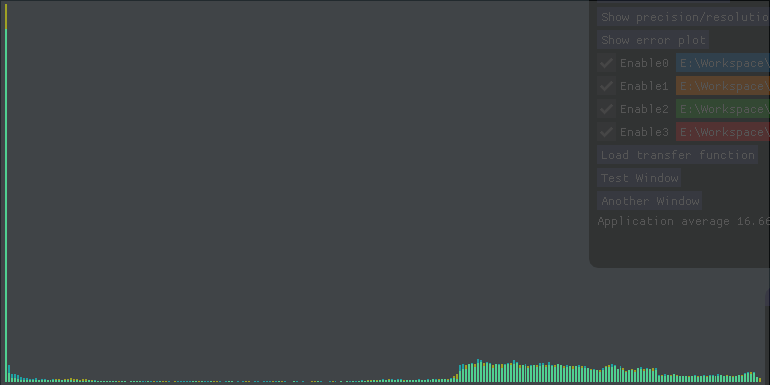
\includegraphics[width=0.48\linewidth]{img/histogram/kflame/histogram.png}}
	\subcaptionbox{\emph{rmse-optimized}}
	{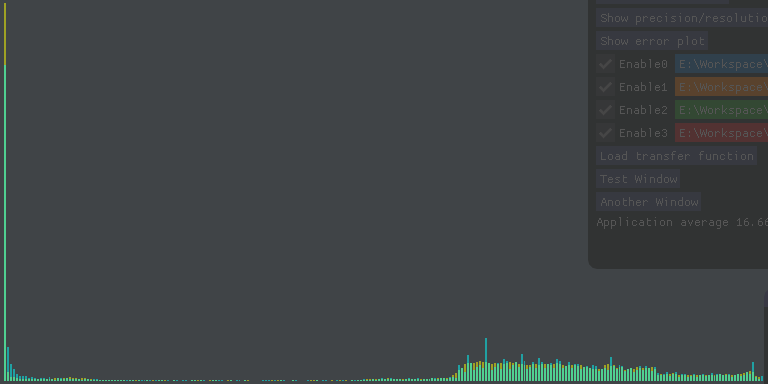
\includegraphics[width=0.48\linewidth]{img/histogram/kflame/rmse.png}}
	\subcaptionbox{\emph{by wavelet norm, slz}}
	{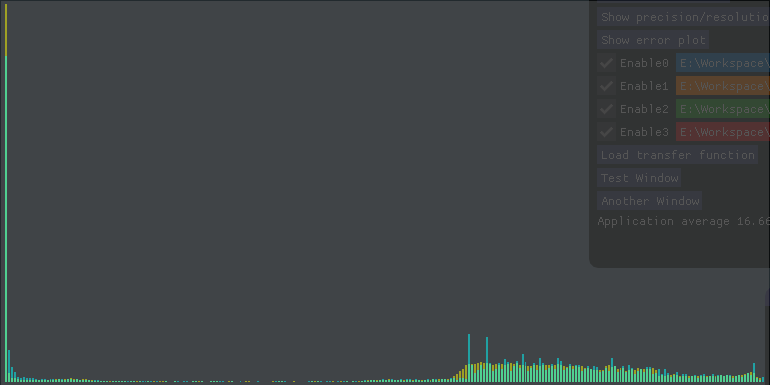
\includegraphics[width=0.48\linewidth]{img/histogram/kflame/wavenorm.png}}
	\subcaptionbox{\emph{histogram signature, slz}}
	{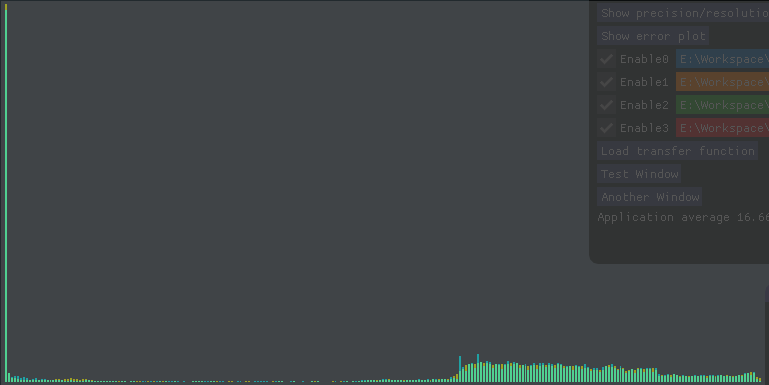
\includegraphics[width=0.48\linewidth]{img/histogram/kflame/signature.png}}
	\subcaptionbox{\emph{histogram-optimized}}
	{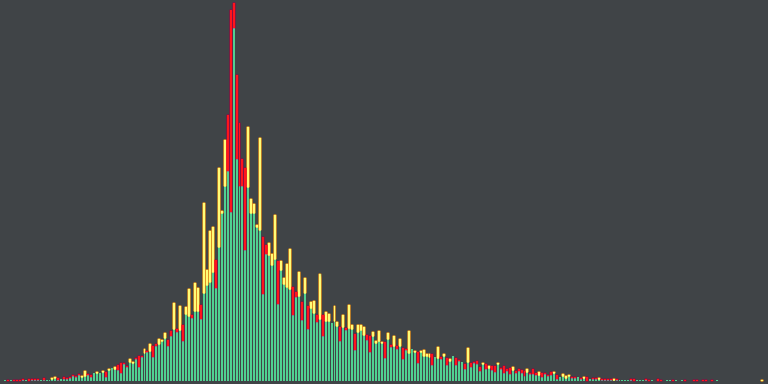
\includegraphics[width=0.48\linewidth]{img/histogram/diffusivity/histogram.png}}
	\subcaptionbox{\emph{rmse-optimized}}
	{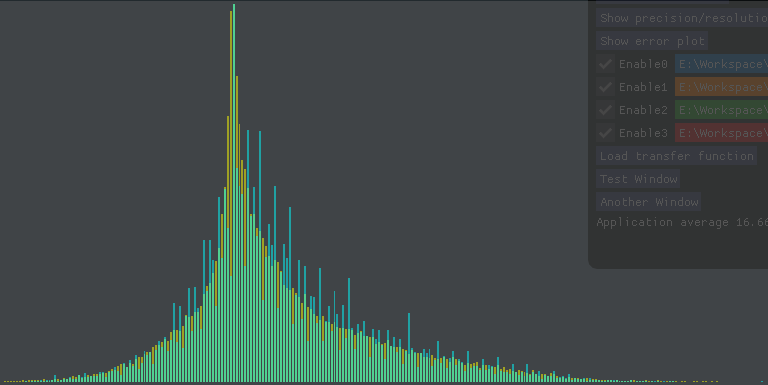
\includegraphics[width=0.48\linewidth]{img/histogram/diffusivity/rmse.png}}
	\subcaptionbox{\emph{by wavelet norm, slz}}
	{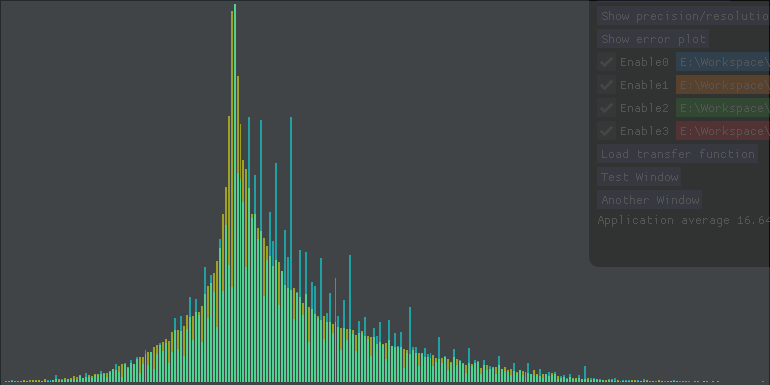
\includegraphics[width=0.48\linewidth]{img/histogram/diffusivity/wavenorm.png}}
	\subcaptionbox{\emph{histogram signature, slz}}
	{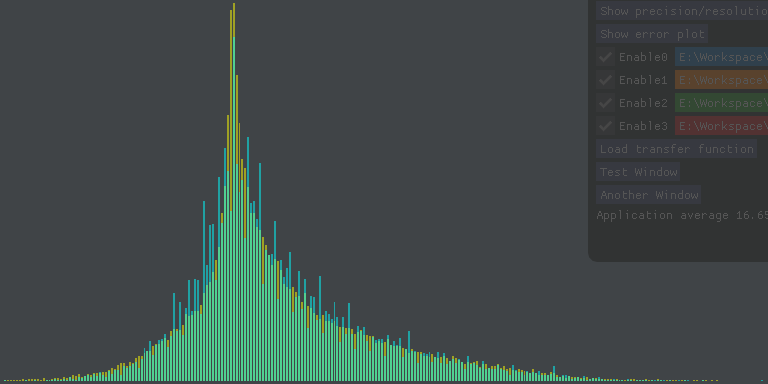
\includegraphics[width=0.48\linewidth]{img/histogram/diffusivity/signature.png}}
	\caption{Histogram comparison. (a,b,c,d) kflame, 0.14 bps. (e,f,g,h) diffusivity, 0.09 bps.}
	\label{fig:histogram-comparison-low-bit-rate}
\end{figure}

Histogram computation is another common 
We compare different error metric for histogram in two figures:
Figure 1: PSNR plot for all histogram streams using different error metrics.

Figure 2: histogram plots for each metric, at some low bit rate

Figure 3: RMSE error between rmse stream and histogram stream for one data set

Figure 4: Histogram error for the  above two streams for the same data set.

To somewhat quantify the differences of two streams, we define the concept of a stream signature, and present the algorithm to compute a signature.

Algorithm. How to compute a stream's signature.

We show the two signatures for rmse and histogram streams for the same data set.

Figure 5: show signature of the two streams

Figure 6: show signatures for different number of bins

Figure 7: Show that we can stream using the histogram signature to get better histogram than rmse